


\thispagestyle{empty} 
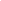
\includegraphics{Images/pixel.png}
\vfill
\parbox[b]{11cm}{\raggedright

\textcopyright {\the\year} Peter W. Brewer\\[2mm] Laboratory of Tree-Ring Research\\ 1215 E. Lowell Street \\
Tucson\\
Arizona 85721. USA.\\[0.5cm] \Telefon\hspace{3mm}+1 520 621 0753 \\ \Letter\hspace{3mm}p.brewer@ltrr.arizona.edu\\[5mm] Compiled: \today\\[10mm]}

{\footnotesize 
Permission is granted to copy, distribute and/or modify this document
under the terms of the GNU Free Documentation License, Version 1.3
or any later version published by the Free Software Foundation;
with no Invariant Sections, no Front-Cover Texts, and no Back-Cover Texts.
A copy of the license is included in the appendix entitled ``GNU Free Documentation License'' (pages \pageref{txt:FDLStart}--\pageref{txt:FDLEnd}).}



\newpage
\pagenumbering{roman}
\setcounter{page}{1}
\thispagestyle{empty} 
{ 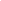
\includegraphics{Images/pixel.png}\\[4cm] 
\hrule 
\vspace{5mm}
\Huge \bfseries \thetitle\\[3mm] 
\large{\thesubtitle}
\vspace{5mm}
\hrule
\vspace{3cm}
}
{
\normalsize
\textbf{By \authornames}\\[0.6cm]
}
{
\vfill
\footnotesize
Compiled: \today
}

\newpage


\tableofcontents


\cleardoublepage
\pagenumbering{arabic} 

\phantomsection
\section*{Preface}
\thispagestyle{empty} 
\addcontentsline{toc}{section}{Preface}

The Tellervo application is primarily designed for the measurement of tree ring widths and the organization and curation of the data, metadata and physical samples for dendrochronological research. It is cross-platform (running on all Java 6 and later enabled operating systems including Windows, MacOSX and Linux) and open-source. It includes support for standard measuring platforms including Velmex, Lintab and Henson.

Tellervo is a substantial rewrite of the original dendro application `Corina' developed at Cornell University since 2000.  Corina itself following an earlier DOS-based version programmed in C, which in turn was derived from a collection of FORTRAN and C utilities.  While Corina was built around a standard file-based data management system, Tellervo uses an object-relational database management system (ORDBMS) and server/client webservice infrastructure based on the Tree Ring Data Standard (TRiDaS).  The application was renamed Tellervo to reflect the substantial changes made from the original Corina code-base. 

This manual is divided into two main sections, the first for users, the second for developers.  Tellervo is open source software (see the details of the license on pages \pageref{txt:licenseStart}--\pageref{txt:licenseEnd}), so you are welcome to inspect and edit the code.  The second part of this manual will help you do that.

Over the years Corina and Tellervo have been developed by: Peter Brewer, Chris Dunham, Aaron Hamid, Dan Girshovich, Ken Harris, Drew Kalina, Rocky Li, Lucas Madar, Daniel Murphy, Robert `Mecki' Pohl and Kit Sturgeon.  We would like to thank the many people that have tested the applications especially: Charlotte Pearson; Carol Griggs; Brita Lorentzen; Jess Herlich; LeAnn Canady; Kate Seufer; Nathan English; and many undergraduate and postgradutes students at Cornell and the Laboratory of Tree-Ring Research, University of Arizona.  

We would also like to thank the College of Arts \& Sciences and the Department of Classics, Cornell University; the Malcolm H.\ Wiener Foundation; and the many patrons of the Malcolm and Carolyn Wiener Laboratory for Aegean and Near Eastern Dendrochronology for their financial support.  

We hope that you find Tellervo useful and look forward to hearing your feedback.  



